\begin{frame}
    \frametitle{Implémentation non naïve de la multiplication de matrices}
    Implémentation tirée du livre \textit{OpenCL Programming Guide}.
    \newline
    Principe:\pause{}
    \begin{itemize}
        \item un \textit{work item} calcule une ligne de la matrice C\pause{}
        \item les \textit{work items} sont regroupés dans différents \textit{work groups}\pause{}
    \end{itemize}
    But: optimiser les mouvements de données.\pause{}
    \vspace{10pt}
    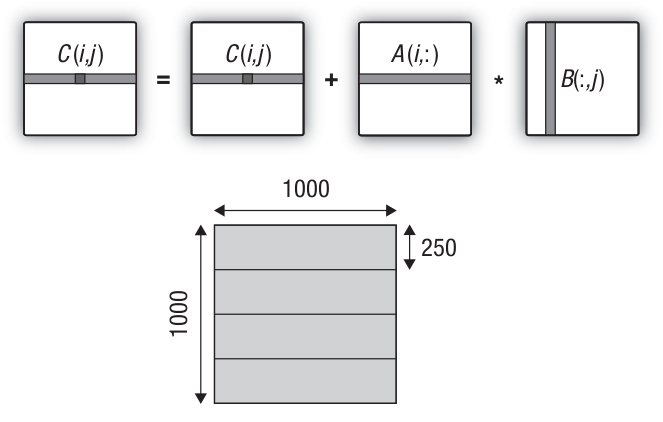
\includegraphics[width=\textwidth]{../resources/non_naive_implementation_principle.png}
\end{frame}

\begin{frame}[fragile,allowframebreaks]
    \frametitle{Implémentation non naïve de la multiplication de matrices}
    \begin{lstlisting}[language=python]
    import numpy as np
    import pyopencl as cl

    N_WORK_GROUPS = 32
    # we keep size which represents a lenght of a line/colunm 
    # by powers of two to be able to divide evenly everything for work groups
    size = next_power_of_two32bit(max([A_dim[0], A_dim[1], B_dim[0], B_dim[1]]))    

    A = np.random.rand(A_dim[0] * A_dim[1]).astype(np.float32)   
    B = np.random.rand(B_dim[0] * B_dim[1]).astype(np.float32)   
    C = np.zeros(A_dim[1] * B_dim[0], dtype=np.float32)

    # our matrices are now of dimensions (size, size)
    A = matrix_resize_with_zeros(A, size)
    B = matrix_resize_with_zeros(B, size)
    C = matrix_resize_with_zeros(C, size)

    A_buffer = cl.Buffer(context, flags=cl.mem_flags.READ_ONLY, size=A.nbytes)
    B_buffer = cl.Buffer(context, flags=cl.mem_flags.READ_ONLY, size=B.nbytes)
    C_buffer = cl.Buffer(context, flags=cl.mem_flags.WRITE_ONLY, size=C.nbytes)

    cl.enqueue_copy(queue, src=A, dest=A_buffer)
    cl.enqueue_copy(queue, src=B, dest=B_buffer)

    kernel_arguments = (A_buffer, B_buffer, C_buffer,
                        # local memory size needs to be passed for
                        # local argument
                        cl.LocalMemory(A[0].nbytes),
                        np.int32(size))

    program.matrix_mult(queue,
                        [size],
                        [size // N_WORK_GROUPS],
                        *kernel_arguments).wait()

    cl.enqueue_copy(queue, src=C_buffer, dest=C)

    matrices_resize_original_dimensions(C, A_dim[0], B_dim[1])
    \end{lstlisting}
\end{frame}

\begin{frame}[fragile]
    \frametitle{Implémentation non naïve de la multiplication de matrices}
    \begin{lstlisting}[language=c]
    /* #define AWRK_SIZE is added by the host program */
    __kernel void matrix_mult(__global float* A,
                              __global float* B,
                              __global float* C,
                              __local float* Bwrk,  /* local memory of b column for work group */
                              const int ncol) {
        int i = get_global_id(0);
        int iloc = get_local_id(0);
        int nloc = get_local_size(0);

        float Awrk[AWRK_SIZE];  /* private memory of a column for work item */

        if (i < ncol) {
            /* copy elements in private memory */
            for (int k = 0 ; k < ncol ; k++) {
                Awrk[k] = A[i * ncol + k];
            }

            for (int j = 0 ; j < ncol ; j++) {
                /* copy elements in local memory */
                for (int k = iloc ; k < ncol ; k = k + nloc) {
                    Bwrk[k] = B[k * ncol + j];
                }
                barrier(CLK_LOCAL_MEM_FENCE);
                float tmp = 0.0;
                for (int k = 0 ; k < ncol ; k++) {
                    tmp += Awrk[k] * Bwrk[k];
                }
                C[i * ncol + j] = tmp;
            }
        }
    }
    \end{lstlisting}
\end{frame}

\begin{frame}
    \frametitle{Implémentation non naïve de la multiplication de matrices}
    Trois genres de mesures:\pause{}
    \begin{itemize}
        \item le temps de copie des \textit{buffers}\pause{}
        \item le temps d'exécution\pause{}
        \item la précision des résultats\pause{}
    \end{itemize}\pause{}
    \vspace{20pt}
    Des matrices carrées de même dimension allant de 10 à 1 500 lignes/colonnes par pas de 10.
\end{frame}

\begin{frame}
    \frametitle{Implémentation non naïve de la multiplication de matrices}
    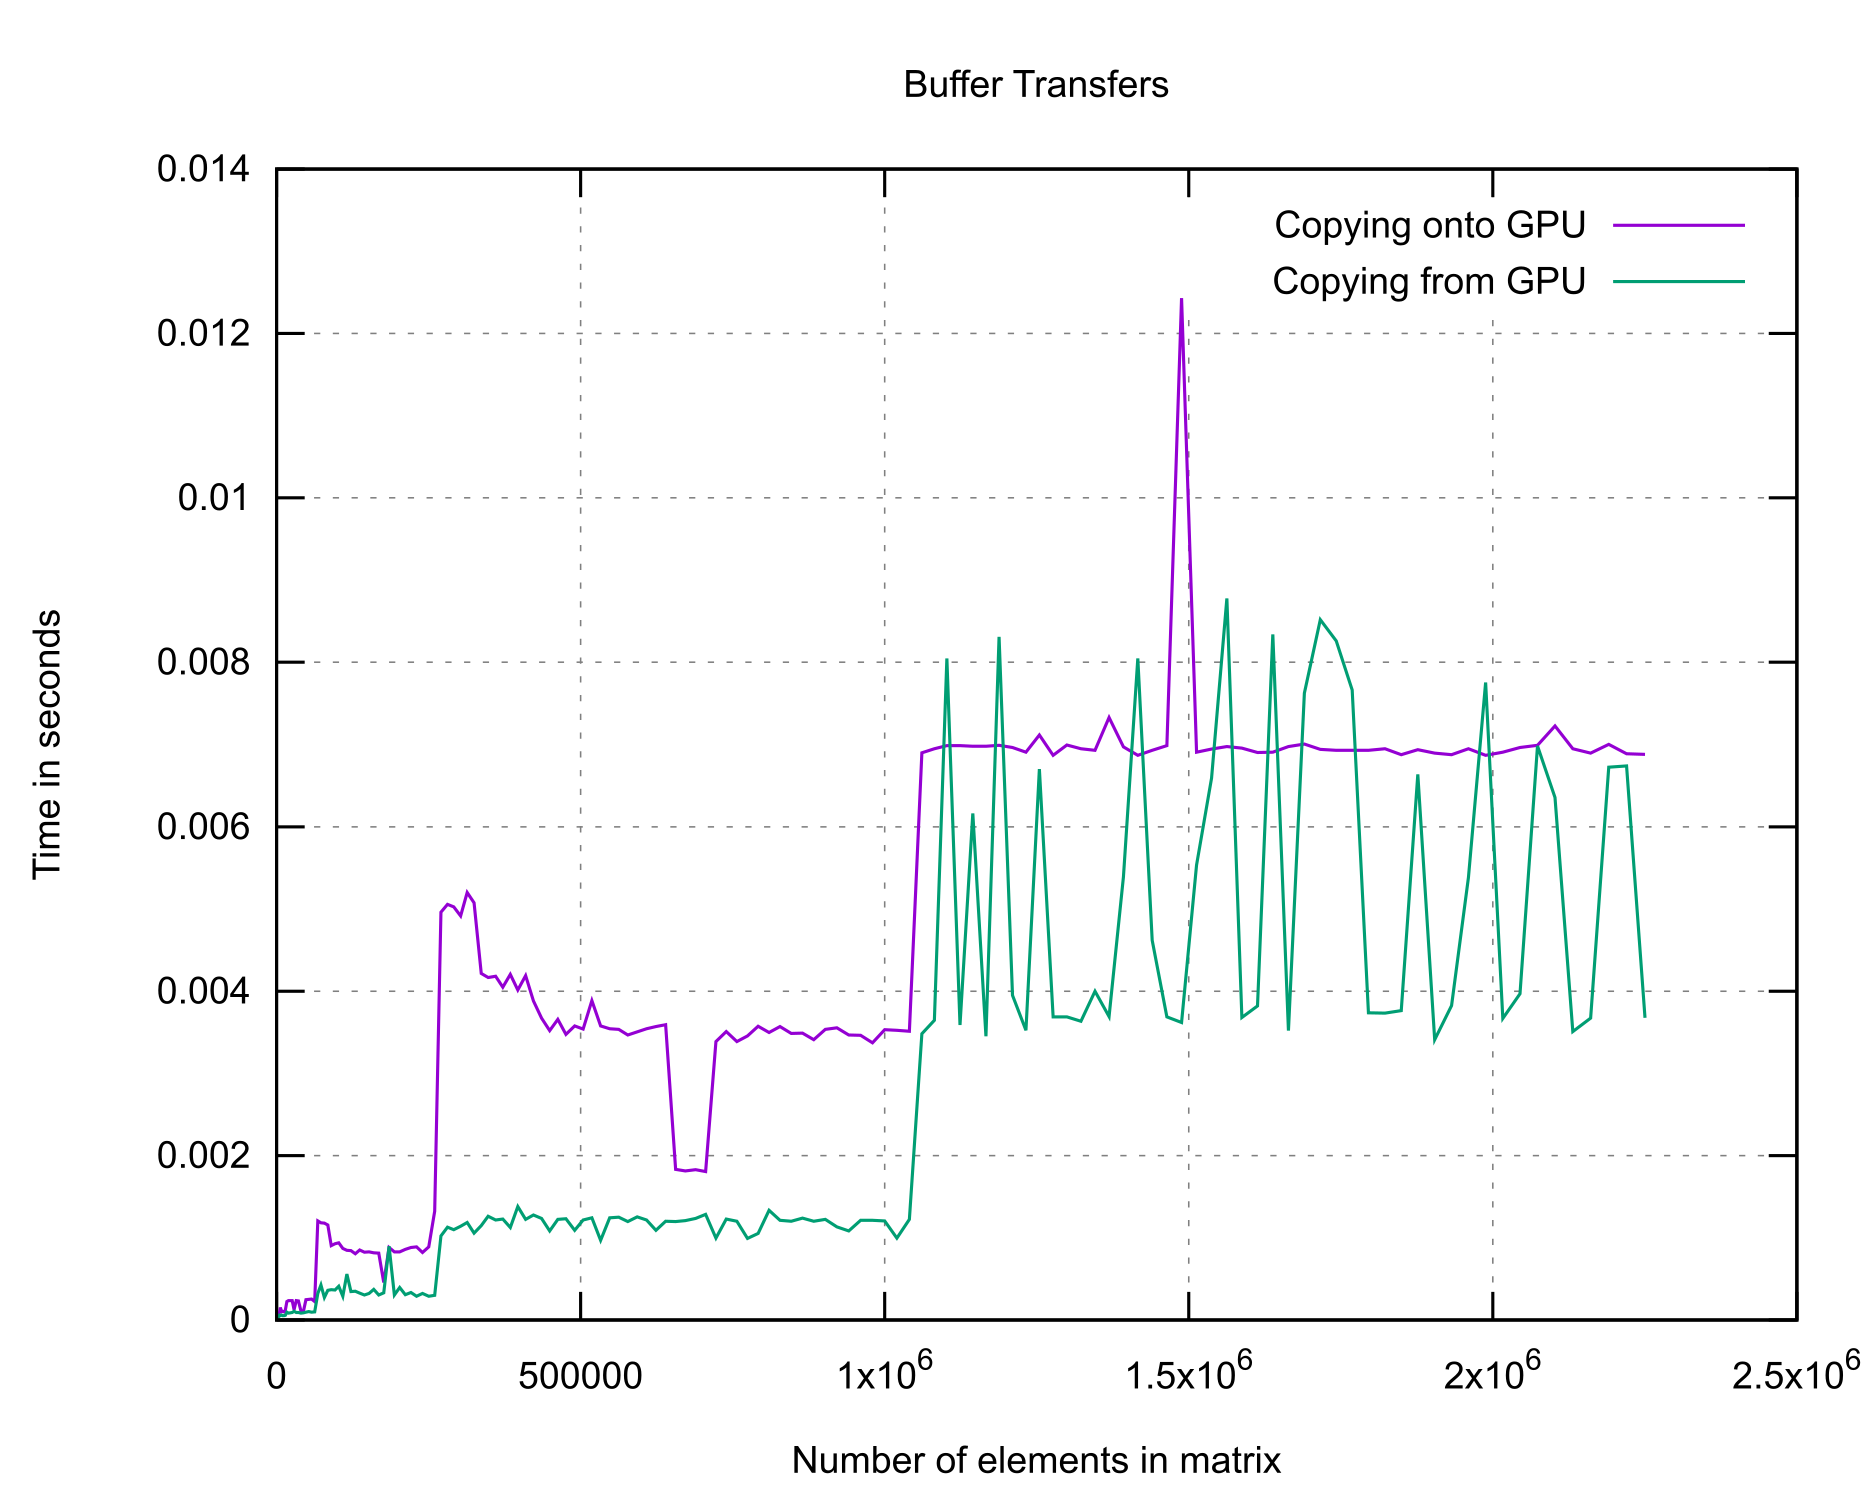
\includegraphics[width=\textwidth]{../resources/buffer_transfer.png}
\end{frame}

\begin{frame}
    \frametitle{Implémentation non naïve de la multiplication de matrices}
    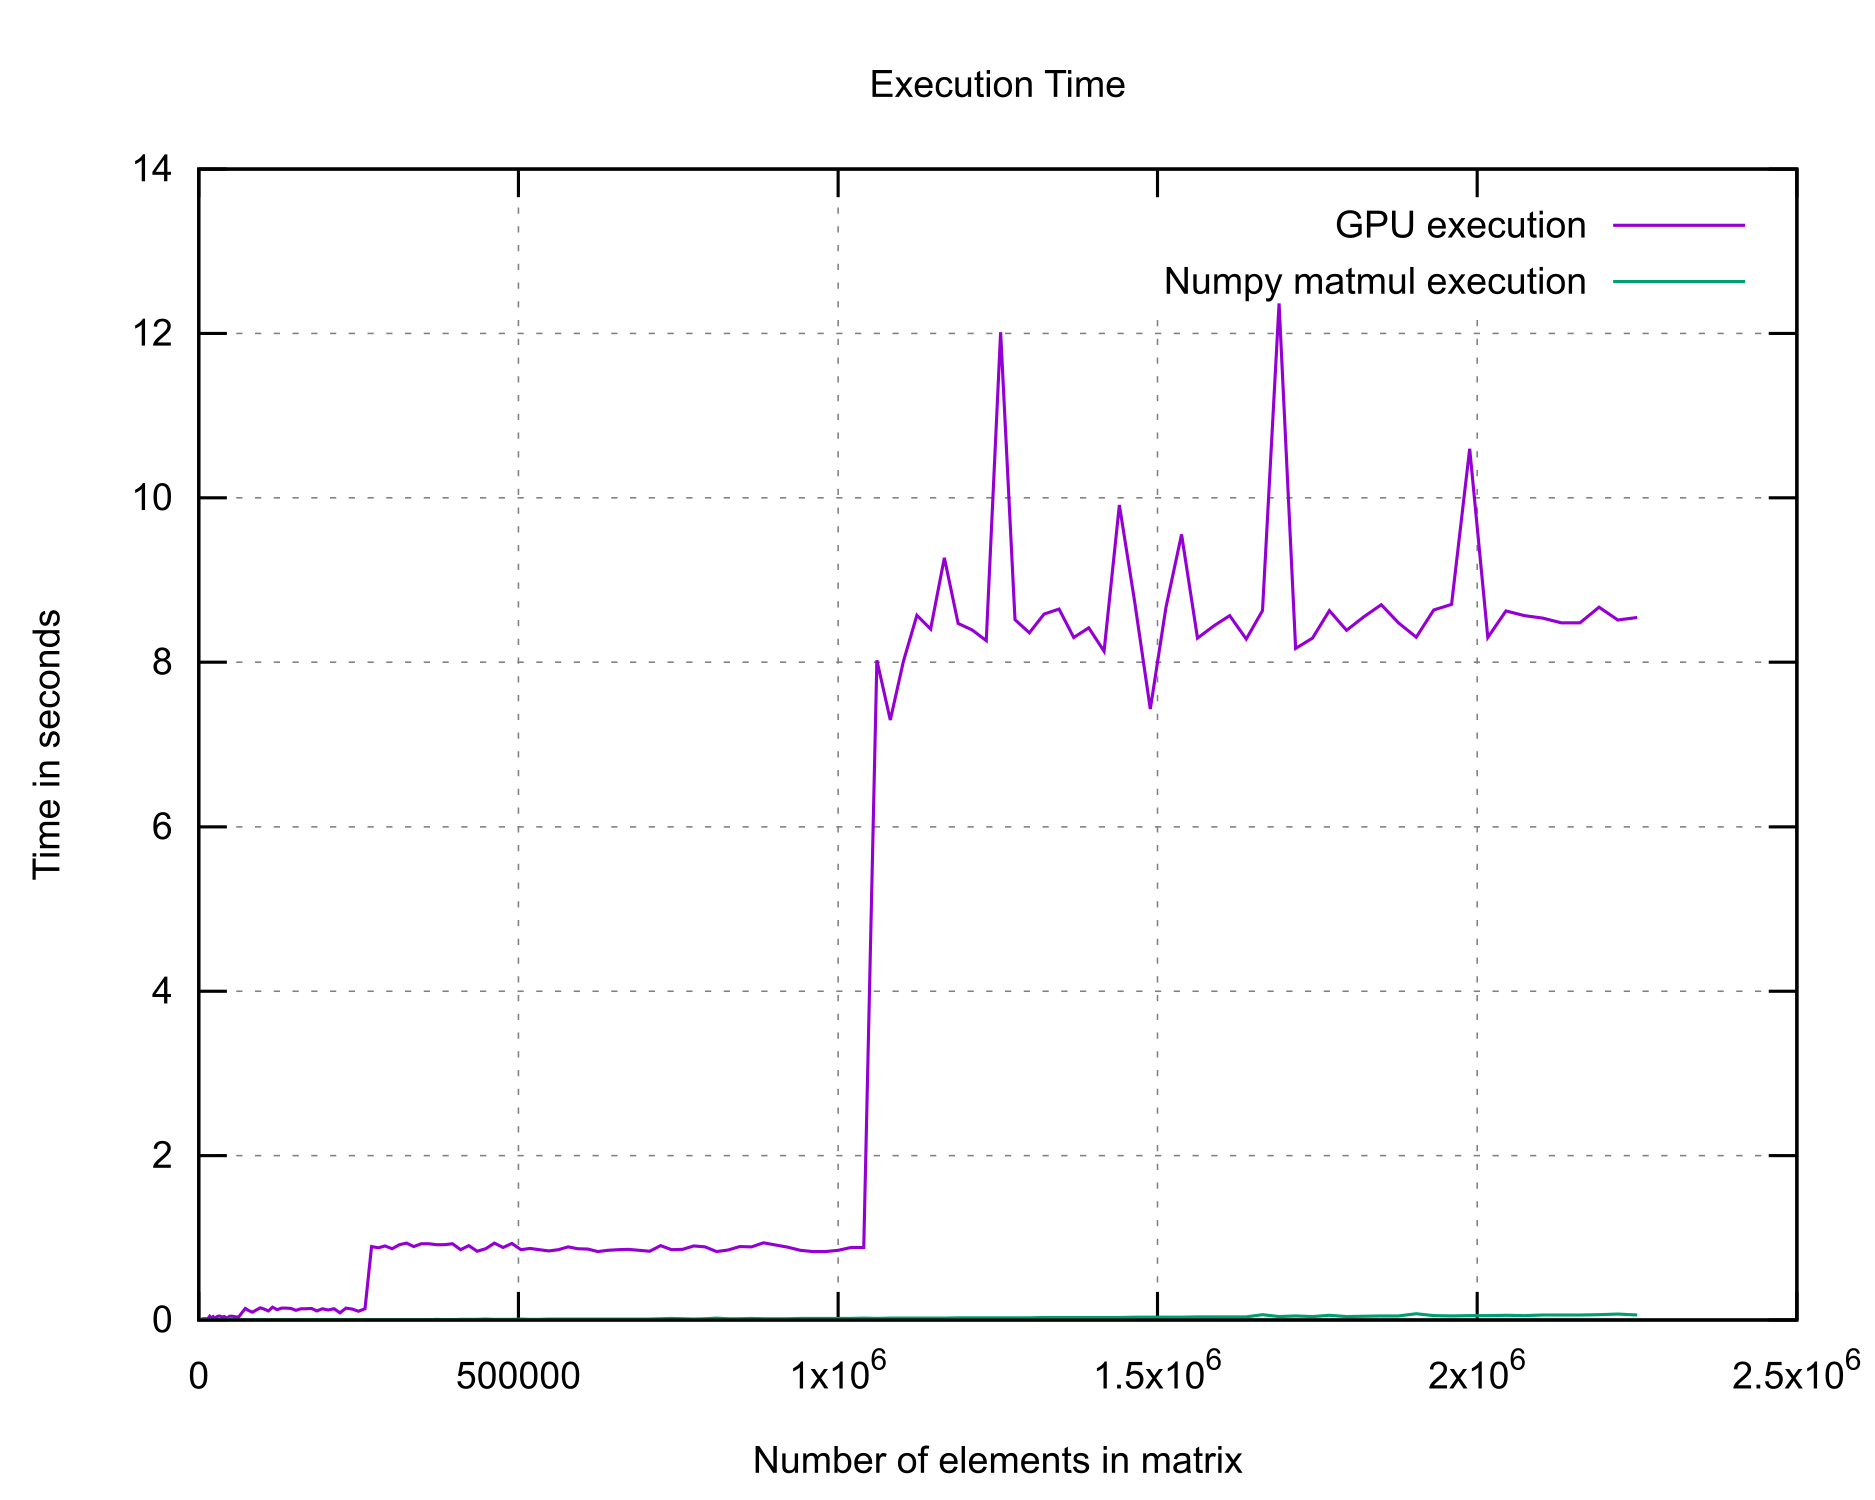
\includegraphics[width=\textwidth]{../resources/execution_time.png}
\end{frame}

\begin{frame}
    \frametitle{Implémentation non naïve de la multiplication de matrices}
    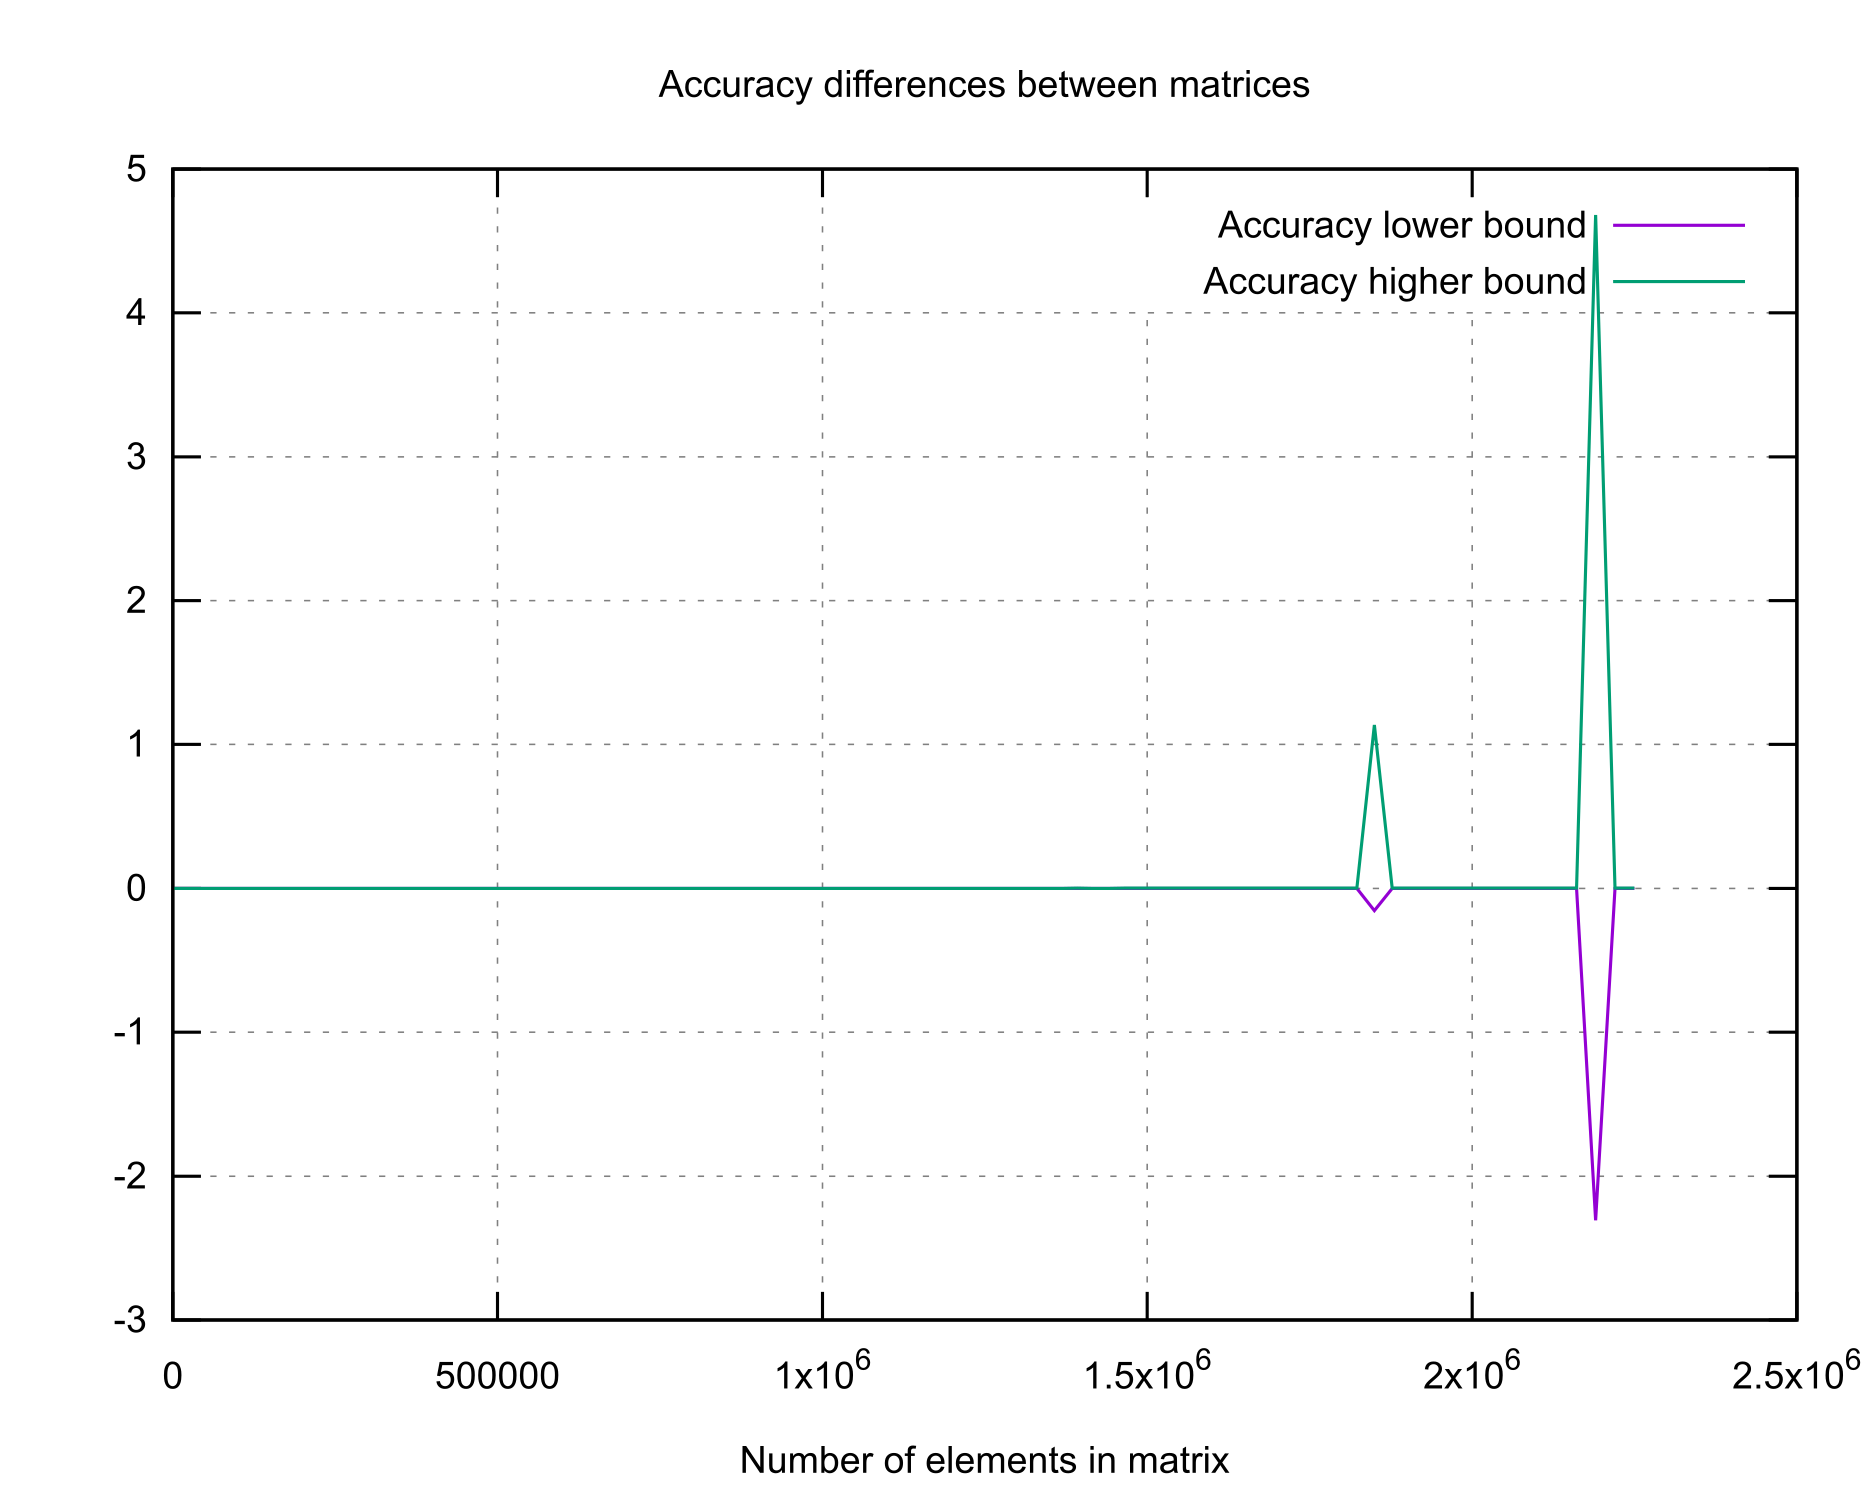
\includegraphics[width=\textwidth]{../resources/float_accuracy.png}
\end{frame}
